\documentclass{beamer}
\usepackage{graphicx}

\usetheme{Dresden}
\setbeamertemplate{navigation symbols}{}

\usepackage{mathtools}
\newcommand{\dd}{\, \text{d}}
\renewcommand{\vec}[1]{\ensuremath{\mathbf{#1}}}
\newcommand{\op}[1]{\ensuremath{\mathbf{#1}}}

\title[HMC]{Implementing Hamiltonian Monte Carlo for Efficent Bayesian Evolutionary Analysis}
\author{Arman Bilge}
\date{2 April 2015}

\begin{document}

    \frame{\titlepage}
    
    \section{Introduction}
    
    \begin{frame}{Bayesian Evolutionary Analysis}
        
        \begin{equation}
            p\left(T \mid D\right)
                \propto \int_\theta p\left(D \mid T,\theta\right)
                p\left(T \mid \theta\right) p\left(\theta\right) \dd\theta
        \end{equation}
        
        $p\left(D \mid T,\theta\right)$ is the Felsenstein tree likelihood. \\
        $p\left(T \mid \theta\right)$ is the tree prior. \\
        $\theta$ are nuisance parameters.
        
    \end{frame}
    
    \section{Methods}
    
    \begin{frame}{The Operators}
        
        \begin{definition}
            $\op{F}\left\{\vec{q},\vec{p}\right\} = \left\{\vec{q},-\vec{p}\right\}$
        \end{definition}
        
        \vfill
        
        \centering
        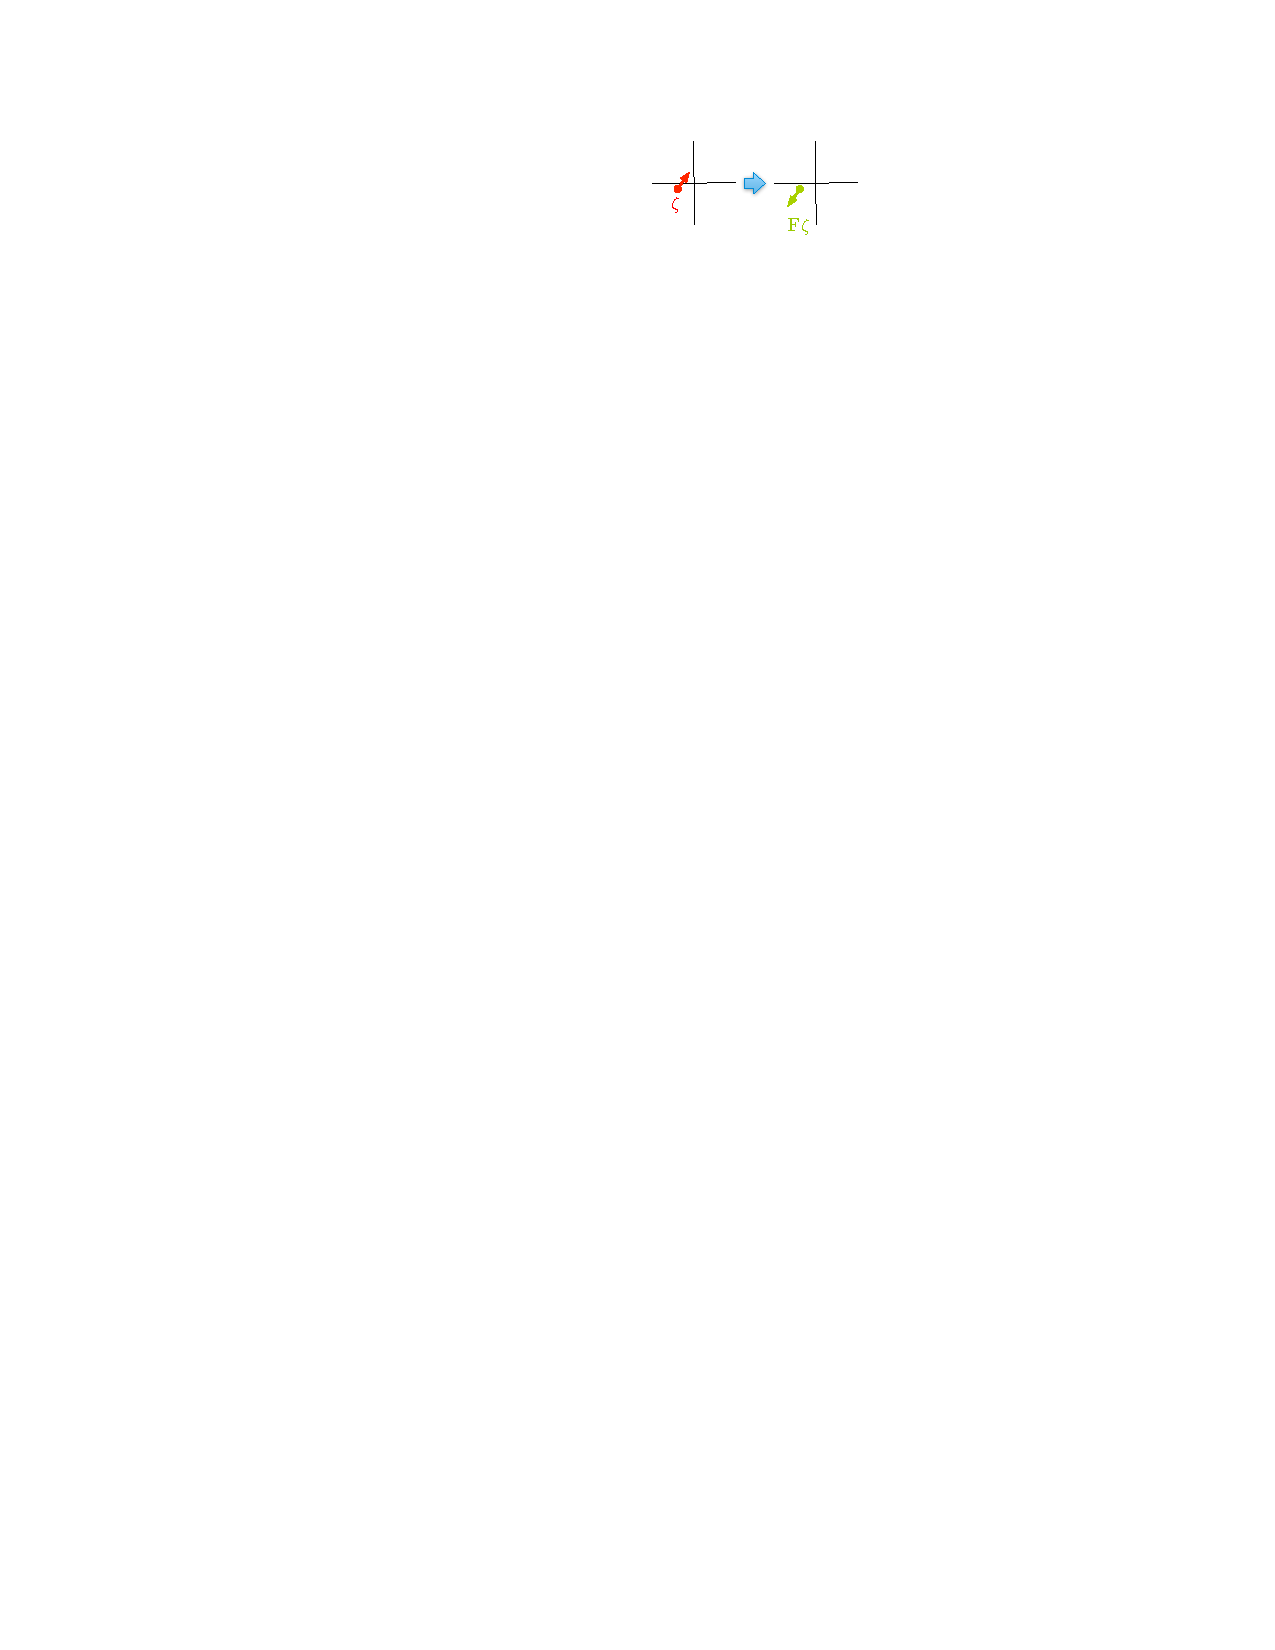
\includegraphics[width=0.75\textwidth]{F.pdf}
        
    \end{frame}

    \begin{frame}{The Operators}
        
        \begin{definition}
            $\op{L}\left\{\vec{q},\vec{p}\right\} = \text{The state after } \epsilon L \text{ time, as approximated by } L \text{ leapfrogs with stepsize } \epsilon$
        \end{definition}
        
        \vfill
        
        \centering
        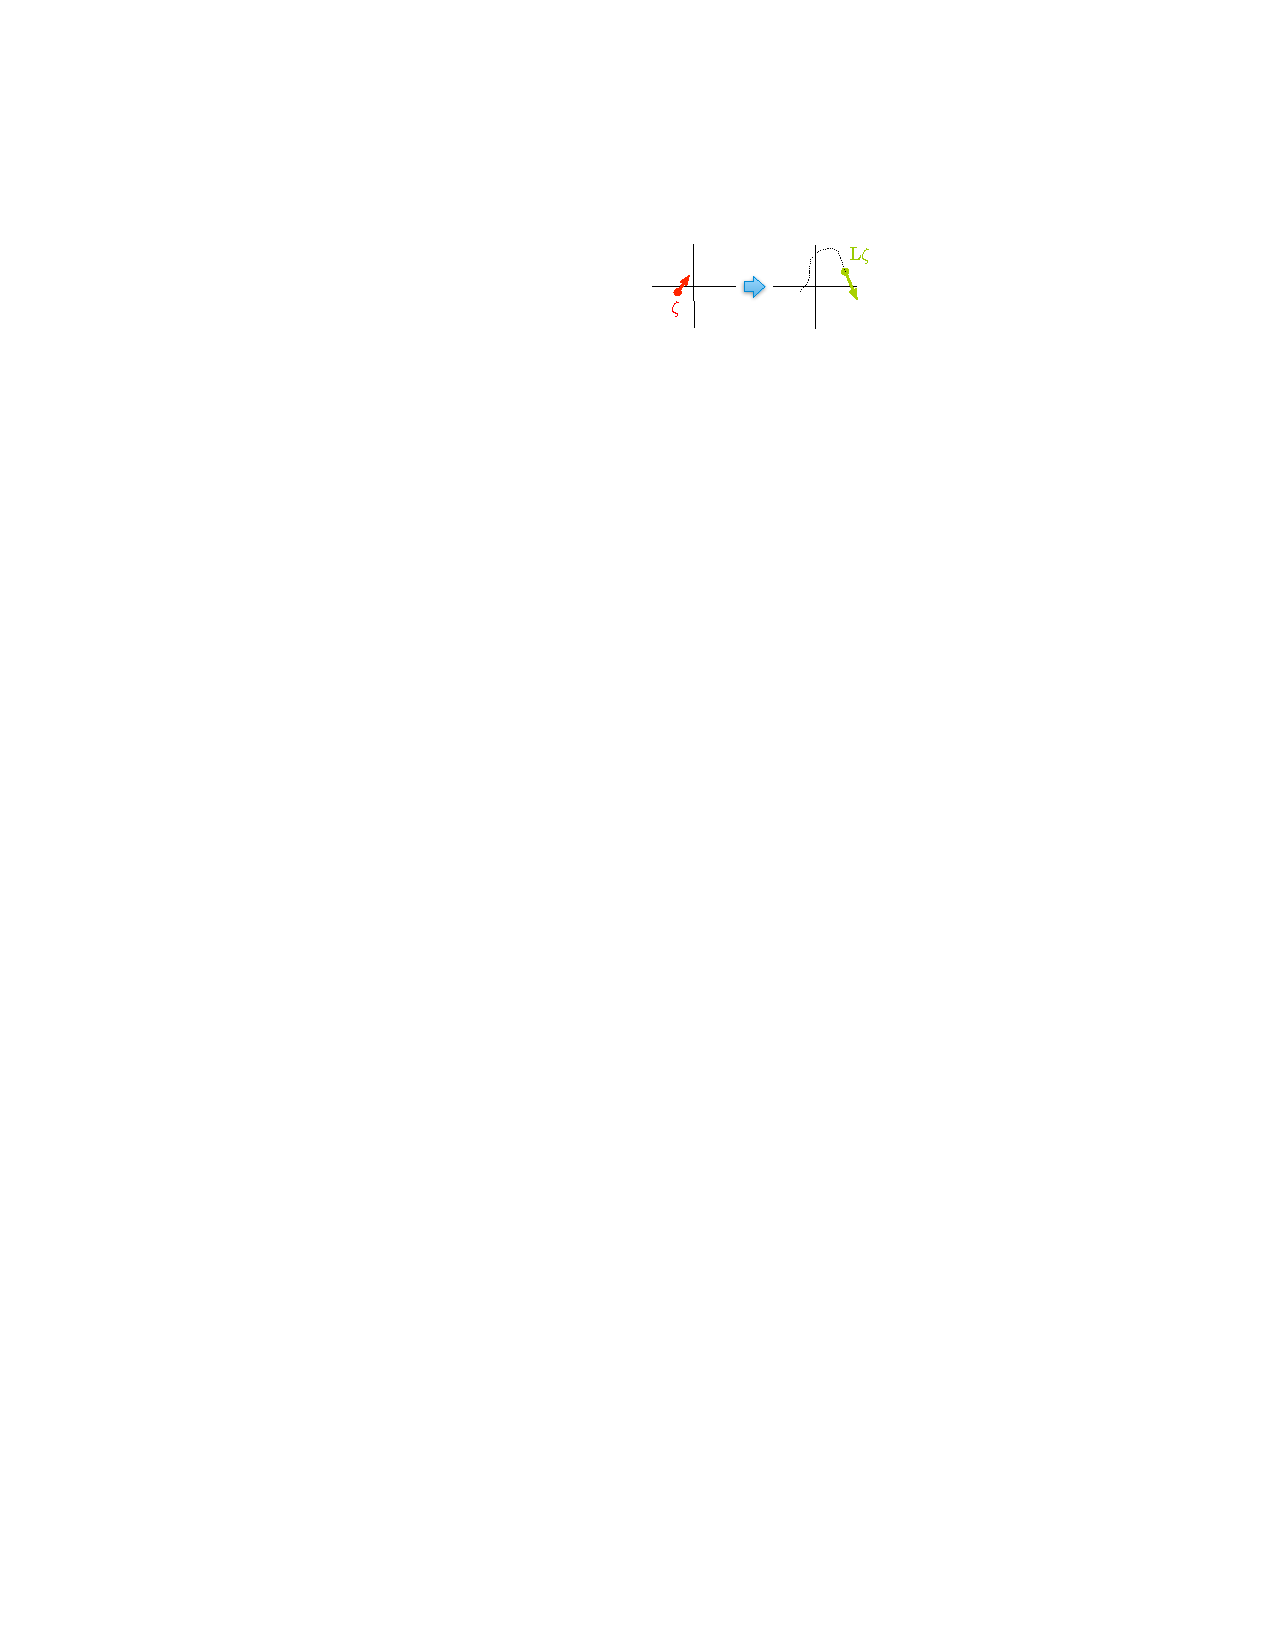
\includegraphics[width=0.75\textwidth]{L.pdf}
        
    \end{frame}
    
\end{document}